% Options for packages loaded elsewhere
\PassOptionsToPackage{unicode}{hyperref}
\PassOptionsToPackage{hyphens}{url}
%
\documentclass[
]{book}
\usepackage{amsmath,amssymb}
\usepackage{lmodern}
\usepackage{iftex}
\ifPDFTeX
  \usepackage[T1]{fontenc}
  \usepackage[utf8]{inputenc}
  \usepackage{textcomp} % provide euro and other symbols
\else % if luatex or xetex
  \usepackage{unicode-math}
  \defaultfontfeatures{Scale=MatchLowercase}
  \defaultfontfeatures[\rmfamily]{Ligatures=TeX,Scale=1}
\fi
% Use upquote if available, for straight quotes in verbatim environments
\IfFileExists{upquote.sty}{\usepackage{upquote}}{}
\IfFileExists{microtype.sty}{% use microtype if available
  \usepackage[]{microtype}
  \UseMicrotypeSet[protrusion]{basicmath} % disable protrusion for tt fonts
}{}
\makeatletter
\@ifundefined{KOMAClassName}{% if non-KOMA class
  \IfFileExists{parskip.sty}{%
    \usepackage{parskip}
  }{% else
    \setlength{\parindent}{0pt}
    \setlength{\parskip}{6pt plus 2pt minus 1pt}}
}{% if KOMA class
  \KOMAoptions{parskip=half}}
\makeatother
\usepackage{xcolor}
\usepackage{color}
\usepackage{fancyvrb}
\newcommand{\VerbBar}{|}
\newcommand{\VERB}{\Verb[commandchars=\\\{\}]}
\DefineVerbatimEnvironment{Highlighting}{Verbatim}{commandchars=\\\{\}}
% Add ',fontsize=\small' for more characters per line
\usepackage{framed}
\definecolor{shadecolor}{RGB}{248,248,248}
\newenvironment{Shaded}{\begin{snugshade}}{\end{snugshade}}
\newcommand{\AlertTok}[1]{\textcolor[rgb]{0.94,0.16,0.16}{#1}}
\newcommand{\AnnotationTok}[1]{\textcolor[rgb]{0.56,0.35,0.01}{\textbf{\textit{#1}}}}
\newcommand{\AttributeTok}[1]{\textcolor[rgb]{0.77,0.63,0.00}{#1}}
\newcommand{\BaseNTok}[1]{\textcolor[rgb]{0.00,0.00,0.81}{#1}}
\newcommand{\BuiltInTok}[1]{#1}
\newcommand{\CharTok}[1]{\textcolor[rgb]{0.31,0.60,0.02}{#1}}
\newcommand{\CommentTok}[1]{\textcolor[rgb]{0.56,0.35,0.01}{\textit{#1}}}
\newcommand{\CommentVarTok}[1]{\textcolor[rgb]{0.56,0.35,0.01}{\textbf{\textit{#1}}}}
\newcommand{\ConstantTok}[1]{\textcolor[rgb]{0.00,0.00,0.00}{#1}}
\newcommand{\ControlFlowTok}[1]{\textcolor[rgb]{0.13,0.29,0.53}{\textbf{#1}}}
\newcommand{\DataTypeTok}[1]{\textcolor[rgb]{0.13,0.29,0.53}{#1}}
\newcommand{\DecValTok}[1]{\textcolor[rgb]{0.00,0.00,0.81}{#1}}
\newcommand{\DocumentationTok}[1]{\textcolor[rgb]{0.56,0.35,0.01}{\textbf{\textit{#1}}}}
\newcommand{\ErrorTok}[1]{\textcolor[rgb]{0.64,0.00,0.00}{\textbf{#1}}}
\newcommand{\ExtensionTok}[1]{#1}
\newcommand{\FloatTok}[1]{\textcolor[rgb]{0.00,0.00,0.81}{#1}}
\newcommand{\FunctionTok}[1]{\textcolor[rgb]{0.00,0.00,0.00}{#1}}
\newcommand{\ImportTok}[1]{#1}
\newcommand{\InformationTok}[1]{\textcolor[rgb]{0.56,0.35,0.01}{\textbf{\textit{#1}}}}
\newcommand{\KeywordTok}[1]{\textcolor[rgb]{0.13,0.29,0.53}{\textbf{#1}}}
\newcommand{\NormalTok}[1]{#1}
\newcommand{\OperatorTok}[1]{\textcolor[rgb]{0.81,0.36,0.00}{\textbf{#1}}}
\newcommand{\OtherTok}[1]{\textcolor[rgb]{0.56,0.35,0.01}{#1}}
\newcommand{\PreprocessorTok}[1]{\textcolor[rgb]{0.56,0.35,0.01}{\textit{#1}}}
\newcommand{\RegionMarkerTok}[1]{#1}
\newcommand{\SpecialCharTok}[1]{\textcolor[rgb]{0.00,0.00,0.00}{#1}}
\newcommand{\SpecialStringTok}[1]{\textcolor[rgb]{0.31,0.60,0.02}{#1}}
\newcommand{\StringTok}[1]{\textcolor[rgb]{0.31,0.60,0.02}{#1}}
\newcommand{\VariableTok}[1]{\textcolor[rgb]{0.00,0.00,0.00}{#1}}
\newcommand{\VerbatimStringTok}[1]{\textcolor[rgb]{0.31,0.60,0.02}{#1}}
\newcommand{\WarningTok}[1]{\textcolor[rgb]{0.56,0.35,0.01}{\textbf{\textit{#1}}}}
\usepackage{longtable,booktabs,array}
\usepackage{calc} % for calculating minipage widths
% Correct order of tables after \paragraph or \subparagraph
\usepackage{etoolbox}
\makeatletter
\patchcmd\longtable{\par}{\if@noskipsec\mbox{}\fi\par}{}{}
\makeatother
% Allow footnotes in longtable head/foot
\IfFileExists{footnotehyper.sty}{\usepackage{footnotehyper}}{\usepackage{footnote}}
\makesavenoteenv{longtable}
\usepackage{graphicx}
\makeatletter
\def\maxwidth{\ifdim\Gin@nat@width>\linewidth\linewidth\else\Gin@nat@width\fi}
\def\maxheight{\ifdim\Gin@nat@height>\textheight\textheight\else\Gin@nat@height\fi}
\makeatother
% Scale images if necessary, so that they will not overflow the page
% margins by default, and it is still possible to overwrite the defaults
% using explicit options in \includegraphics[width, height, ...]{}
\setkeys{Gin}{width=\maxwidth,height=\maxheight,keepaspectratio}
% Set default figure placement to htbp
\makeatletter
\def\fps@figure{htbp}
\makeatother
\setlength{\emergencystretch}{3em} % prevent overfull lines
\providecommand{\tightlist}{%
  \setlength{\itemsep}{0pt}\setlength{\parskip}{0pt}}
\setcounter{secnumdepth}{5}
\usepackage{booktabs}
\ifLuaTeX
  \usepackage{selnolig}  % disable illegal ligatures
\fi
\usepackage[]{natbib}
\bibliographystyle{apalike}
\IfFileExists{bookmark.sty}{\usepackage{bookmark}}{\usepackage{hyperref}}
\IfFileExists{xurl.sty}{\usepackage{xurl}}{} % add URL line breaks if available
\urlstyle{same} % disable monospaced font for URLs
\hypersetup{
  pdftitle={DFI Cutoffs: A Tutorial},
  pdfauthor={Melissa G Wolf; Dan McNeish},
  hidelinks,
  pdfcreator={LaTeX via pandoc}}

\title{DFI Cutoffs: A Tutorial}
\author{Melissa G Wolf \and Dan McNeish}
\date{2023-01-22}

\begin{document}
\maketitle

{
\setcounter{tocdepth}{1}
\tableofcontents
}
\hypertarget{introduction}{%
\chapter*{Introduction}\label{introduction}}
\addcontentsline{toc}{chapter}{Introduction}

Confirmatory factor analysis (CFA) is a commonly used statistical method in the social sciences. Although these models have been used for over a century, debate remains about how to evaluate the fit of factor models. Recently, we proposed the use dynamic fit index (DFI) cutoffs to evaluate model fit \citep{mcneish_dynamic_2021, mcneish_dynamic_2022} and introduced a corresponding Shiny application to facilitate their use \citep{wolf_dynamic_2020}.

This book was written as a tutorial for applied psychologists that are interested in using the \href{www.dynamicfit.app}{DFI Shiny App} to compute model specific cutoffs for their CFA models. We wrote this to make DFI cutoffs more accessible to everyone, especially those that use SPSS Amos and Mplus.

In this book, we will walk through 12 commonly asked questions about DFI cutoffs and use an applied example to demonstrate how to use the Shiny app to calculate them. For R users, DFI cutoffs are also available on \texttt{CRAN} under the package \texttt{dynamic} \citep{R-dynamic}.

\begin{Shaded}
\begin{Highlighting}[]
\FunctionTok{install.packages}\NormalTok{(}\StringTok{"dynamic"}\NormalTok{)}
\FunctionTok{library}\NormalTok{(dynamic)}
\end{Highlighting}
\end{Shaded}

\hypertarget{fit-types}{%
\chapter{What are the different types of model fit?}\label{fit-types}}

There are two types of global model fit in CFA: exact fit and approximate fit. Exact fit is a test of model fit in that it compares a test statistic to a probability distribution to calculate a \(p\)-value, while an approximate fit index can be thought of as an effect size measure that quantifies the degree of misfit in the model. Both are derived from the amount of overall misfit in the model, where misfit is defined as the difference between the model-implied variance-covariance matrix (e.g., the user's path diagram) and the data-generated variance-covariance matrix (i.e., the observed relationships in the user's data).

The most commonly used test of \textbf{exact fit} is the \({\chi}^2\) test, although others can be used as well \citep[see][]{mcneish_should_2020}. Tests of exact fit are concerned with the presence of misfit (of any kind) anywhere in the variance-covariance matrices. The \({\chi}^2\) test is a test of exact fit because the null hypothesis is that the model-implied variance-covariance matrix exactly matches the data-generated variance-covariance matrix. If the \({\chi}^2\) test is significant, researchers have evidence to suggest that the model does not exactly fit the data. As such, the \({\chi}^2\) test is the strictest way to evaluate model fit and test psychological theory \citep{hayduk_testing_2007}.

The most used \textbf{approximate fit} indices are the standardized root mean square residual (SRMR), root mean square error of approximation (RMSEA), and the comparative fit index (CFI). There are no probability distributions or p-values associated with these indices, and thus they are not tests of fit but rather a way to evaluate the amount of misfit in the model (e.g., to determine if the misfit is trivial or substantial). In other words, approximate fit indices are different from tests of exact fit because they are concerned with quantifying the degree of misfit in the model. The SRMR is derived from the residual correlation matrix (i.e., the difference between the model-implied variance-covariance matrix and the data-generated variance-covariance matrix) and can be thought of as the average magnitude of the residuals. The RMSEA is derived from the \({\chi}^2\) statistic but differs in that it includes a parsimony correction (i.e., it rewards simpler models with stronger theory that restrict more paths to 0). The CFI is the ratio of the model-reported \({\chi}^2\) and the baseline \({\chi}^2\) and can thus be thought of as the relative improvement in model fit. Lower values of SRMR and RMSEA are indicative of better fit while higher values of the CFI are indicative of better fit \citep{brown_confirmatory_2015}.

The last type of model fit is localized area of fit. In contrast to an overall evaluation of global fit, \textbf{local fit} is an investigation of each cell of the variance covariance matrix to diagnose any areas of strain in the model. This is often done to probe the source of misfit after finding a significant \({\chi}^2\) statistic or a value of an approximate fit index that is indicative of substantial misfit. Still, good global fit can mask local misfit and thus it may be prudent to check regardless of global model fit. Although local fit is discussed at length in introductory textbooks for factor analysis \citep{brown_confirmatory_2015, kline_principles_2011}, it is often not presented in journal articles.

Briefly, local fit can be investigated by probing the residual correlation matrix for extreme cases or by consulting modification indices for modifications that would substantially reduce the \({\chi}^2\) statistic \citep{kline_principles_2011}. Even if an extreme value is found, the model should not be changed unless the revisions are supported theoretically. There are several reasons for this. The first is that the modifications suggested by the software are derived statistically and may substantially alter the theory behind the initial model. Secondly, the misfit may be sample-specific and thus may not generalize to other samples. Third, there is no guarantee that a modification will resolve misfit and could instead lead a researcher down a rabbit hole akin to p-hacking. Fourth, it is difficult to know if misfit is due to an issue with the theory about the internal structure or one or more of the items. As such, any modifications should be justified theoretically and qualitatively.

\hypertarget{fit-weaknesses}{%
\chapter{What are the weaknesses of the current approaches to evaluate model fit?}\label{fit-weaknesses}}

In terms of \textbf{exact fit}, the \({\chi}^2\) test does not perform as well in small samples and may also be overly sensitive to minor misspecifications at large sample sizes \citep{browne_alternative_1992, hu_can_1992}. Additionally, with extremely small samples and smaller loadings, the \({\chi}^2\) test can be underpowered and unable to detect misfit \citep{mcneish_thorny_2018}. Some models (such as bifactor models) inherently have a higher ``fit propensity'', meaning that they are more likely to fit the data regardless of the true nature of the data generating model \citep{bonifay_complexity_2017, bonifay_three_2017, preacher_quantifying_2006}. Further, even if one does find a non-significant p-value for a \({\chi}^2\) test with a reasonable sample size, this does not guarantee that the true model has been recovered as there are often multiple equivalent models that can fit the data \citep{hayduk_seeing_2014}. As such, all modeling decisions should have strong theoretical grounding.

Unlike the \({\chi}^2\) test, \textbf{approximate fit} indices do not have a corresponding p-value. Given that these indices essentially function as effect size measures that capture the degree of misfit in the model, the difficulty lies in how to interpret them and which cutoff values to use (if any). Researchers often rely on a set of fixed cutoff values derived from a simulation study conducted by Hu and Bentler \citeyearpar{hu_cutoff_1999}, which has over 96,000 citations as of 2022. This simulation study produced the well-known cutoff values of SRMR \textless{} .08, RMSEA \textless{} .06, and CFI \textgreater{} .95. However, interpretations of the results from simulations studies are limited to the conditions sampled in the simulation study. Hu and Bentler manipulated the sample size (from 250 -- 5000), the number and type of misspecifications (omitted crossloadings and omitted factor covariances), and the normality of the factors and errors. However, they did not manipulate the number of factors (3), the number of items (15), the magnitude of the factor loadings (.7 - .8), or the model type (single level CFA estimated using maximum likelihood estimation).

Several studies have demonstrated that these fixed cutoff values cannot reliably be extrapolated to other model subspaces (e.g., one-factor models, multi-factor models with stronger or weaker loadings, or models with fewer or greater numbers of items or factors). In other words, if a researcher evaluates the fit of a single-level CFA model that does not have 15 items, 3 factors, and a sample size between 250 -- 5000, the cutoff values derived from Hu and Bentler's study cannot be used to reliably determine if there is substantial misfit in the model \citep{mcneish_dynamic_2021}. Most concerning is the ``reliability paradox'' which stipulates that lower loadings (e.g., a smaller reliability coefficient) are associated with ``better'' values of approximate fit indices \citep{hancock_reliability_2011, heene_masking_2011, marsh_search_2004, mcneish_thorny_2018, saris_testing_2009}. In other words, holding all else equal, as factor loadings decrease, the SRMR and the RMSEA will also decrease, mistakenly leading researchers to conclude that less reliable models fit the data better (when compared to a set of fixed cutoff values). If Hu and Bentler had varied the factor loadings in their original simulation study, it is possible that they would have been unable to recommend a set of fixed cutoff variables since fit indices are so sensitive to loading magnitude.

\hypertarget{why-dfi}{%
\chapter{Why should I use DFI cutoffs instead?}\label{why-dfi}}

Hu and Bentler's approach to quantifying the degree of misspecification in a model was sensible; the problem lies with the interpretation of the fixed cutoff values \citep{millsap_structural_2007, pornprasertmanit_monte_2013}. The first problem is the extrapolation of this fixed set of cutoffs to conditions outside of the ones sampled in their original simulation. Secondly, because Hu and Bentler presented a single set of cutoffs, researchers were inadvertently encouraged to incorrectly treat misfit as a binary decision akin to a test of model fit (e.g., either the model fits well, or it does not). However, the only test of model fit is a test of exact fit; approximate fit indices are useful primarily because they can help researchers judge the extent to which the misfit in their model may be trivial or substantial.

DFI cutoffs are an improvement over the traditional fixed cutoff values because they address both of the issues raised above. DFI cutoffs are tailored to the user's specific model, which alleviates the first problem of improper extrapolation. Researchers can think of DFI cutoffs as ``if Hu and Bentler had used my exact model for their simulation study, these are the cutoff values that they would have published''. Unlike the traditional fixed cutoffs, DFI cutoffs (when available) are accurate for the user's model and can reliably distinguish between a correctly specified model and an incorrectly specified model. In this sense, DFI cutoffs can be thought of as analogous to a custom power analysis (albeit one that is quite simple to conduct).

Secondly, the DFI algorithm is written to return a series of custom cutoff values that range from trivial misfit to substantial misfit. This addresses the second problem of improper interpretation because it encourages researchers to treat misfit as a continuum or a spectrum rather than a binary decision of ``good'' or ``bad''. Because there is less finality associated with an interpretation of model fit when a series of cutoffs are used, the DFI approach also encourages researchers to properly reconceptualize model fit as only one type of validity evidence rather than the crux of validity \citep{aera_apa_ncme_standards_2014}. As such, if a researcher found evidence of trivial misfit according to the DFI cutoffs, they could still potentially defend the use of their scale if they have other sources of evidence of validity in support of its use (while still acknowledging that if the χ2 test is significant then the model does not exactly fit the data).

\hypertarget{algorithm}{%
\chapter{How does the DFI algorithm work?}\label{algorithm}}

The DFI algorithm follows Hu and Bentler's \citeyearpar{hu_cutoff_1999} approach to model misspecification in that it simulates a distribution of fit indices from a correctly specified model and a misspecified model and then chooses a cutoff value that distinguishes between the two distributions. Hu and Bentler created their misspecified models by omitting one or two cross-loadings from a three-factor model (the ``complex'' condition; see Figure \ref{fig:hb}) and by omitting one or two factor correlations from the same three-factor model (the ``simple'' condition). The DFI algorithm mimics this approach by making the user's model both the data generating model and the analytic model (this is the true condition). In the misspecified condition(s), the analytic model remains the user's model, but a series of misspecifications are added to the data generating model (in line with the conventions established by Hu and Bentler). Readers interested in understanding the DFI algorithm in depth should consult McNeish and Wolf \citetext{\citeyear{mcneish_dynamic_2021}; \citeyear{mcneish_dynamic_2022}}.

\begin{figure}

{\centering 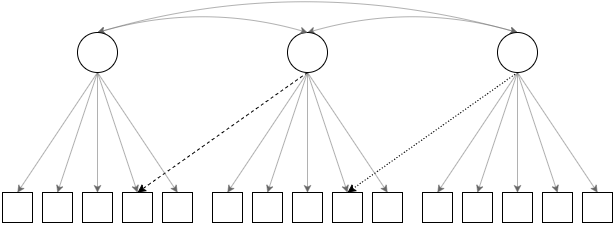
\includegraphics{hb path diagram} 

}

\caption{A path diagram of the model misspecifications used by Hu and Bentler (1999). The true data generating model has all of the loadings. The minor misspecification condition omits the loading with the dashed line from the data generating model, and the major misspecification condition omits both the dashed line and the dotted line from the data generating model. The analytic model is the same for all conditions.}\label{fig:hb}
\end{figure}

\hypertarget{multi-factor-models}{%
\section{Multi-Factor Models}\label{multi-factor-models}}

For multi-factor models, the DFI algorithm creates \(f\)-1 levels of misspecifications, where \(f\) is the number of factors in the model. As such, a two-factor model will have one level of misspecification, while a six-factor model will have five levels of misspecification. The misspecification follows Hu and Bentler's approach of omitting a cross-loading with a magnitude equivalent to the lowest loading in the model from the factor with the highest reliability. For example, the Level 1 misspecification will omit one cross-loading with a magnitude equivalent to the lowest loading, while the Level 2 misspecification will omit both the Level 1 cross-loading and an additional cross-loading with a magnitude equivalent to the second lowest loading in the model. The magnitude of the loading that is omitted can be found in the Info tab of the app and will be returned by default in the R package.

\hypertarget{one-factor-models}{%
\section{One-Factor Models}\label{one-factor-models}}

The algorithm for one-factor models is unique in that it cannot exactly follow the approach established by Hu and Benter \citeyearpar{hu_cutoff_1999} because it is impossible to omit factor correlations or cross-loadings in a one-factor model. As such, the DFI algorithm employs an approach inspired by Shi \& Maydeu-Olivares \citeyearpar{shi_effect_2020} of omitting residual correlations to create a misspecified model. One-factor models have three levels of misspecification , where Level 1 has approximately 1/3rd of items with an omitted residual correlation of .3, Level 2 has approximately 2/3rds of items with an omitted residual correlation of .3, and Level 3 has omitted residual correlations of .3 from all items. As such, the DFI algorithm for the one-factor model is standardized such that the number of items with an omitted residual correlation is proportional to the total number of items in the model, making it easier to compare degree of misfit across models.

\hypertarget{calculate}{%
\chapter{How do I calculate DFI cutoffs?}\label{calculate}}

DFI cutoffs can easily be computed using the free, open source, web-based Shiny application, accessible at \url{www.dynamicfit.app}. The app has a simple, user-friendly, point-and-click interface, which requires no knowledge of coding to operate. The user need only enter their model statement with standardized loadings (see Chapter \ref{model} for more details) and their sample size. Behind the scenes, the Shiny app will use R to run a series of Monte Carlo simulations to return a continuum of cutoff values tailored to the user's individual model. R users who wish to bypass the app can instead make use of the corresponding R package \texttt{dynamic}, available on \texttt{CRAN}, which will return the same results as the web application.

\hypertarget{applied-example}{%
\section{Applied Example}\label{applied-example}}

Computing DFI cutoffs is a post-hoc endeavor; in other words, users must first run their CFA model to get some of the information that is necessary to calculate custom fit index cutoffs. Thus, to make this tutorial easier to follow, we introduce an applied example which will be used throughout the rest of the paper. The data comes from a popular personality assessment commonly referred to as the ``Big Five'', which was provided by the Open Source Psychometrics Project \citep{goldberg_development_1992}. We will use the 10-item ``extraversion'' factor to compute DFI cutoffs for a one-factor model (see Figure \ref{fig:extraversion}).

\begin{figure}

{\centering 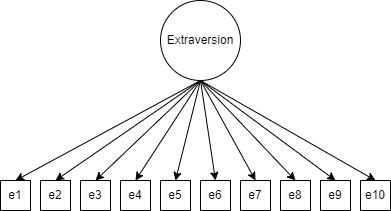
\includegraphics{extraversion path diagram} 

}

\caption{The one-factor model used for the demonstration in this tutorial (n = 1,222).}\label{fig:extraversion}
\end{figure}

To use the Shiny application, researchers should visit the website and select the app that corresponds to their model type. In this case, we will select the one-factor CFA application (see Figure \ref{fig:one}). The app description states that only two pieces of information are needed: (1) the user's standardized loadings from the fitted model, and (2) the sample size. The standardized loadings will be used to create the model statement which will be uploaded to the app to compute the custom DFI cutoffs (see Chapter \ref{model}). The function in the R package \texttt{dynamic} that corresponds to the one-factor CFA app is \texttt{cfaOne}.

\begin{figure}

{\centering 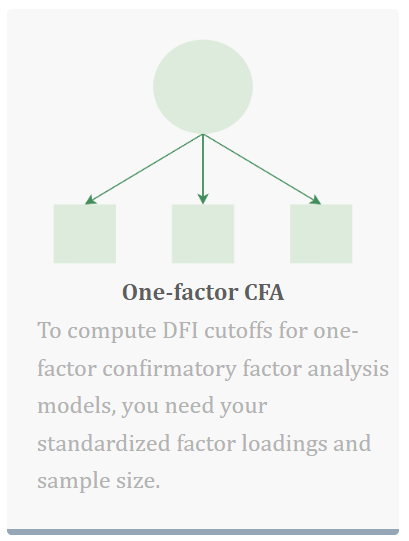
\includegraphics[width=0.4\linewidth]{one factor app} 

}

\caption{The one-factor CFA application on www.dynamicfit.app.}\label{fig:one}
\end{figure}

\hypertarget{model}{%
\chapter{What does a model statement look like?}\label{model}}

After opening the one-factor CFA app, users are prompted to enter two pieces of information: (1) their sample size, and (2) their model statement (see Figure \ref{fig:inputs}). The model statement is created using the standardized loadings from the user's fitted model (i.e., the results from the CFA model that the user wants to calculate DFI cutoffs for). These will be found in the software output that was used to run the original CFA model. We will walk through an example from Mplus and Amos using the Extraversion factor from the Big 5 dataset provided.

\begin{figure}

{\centering 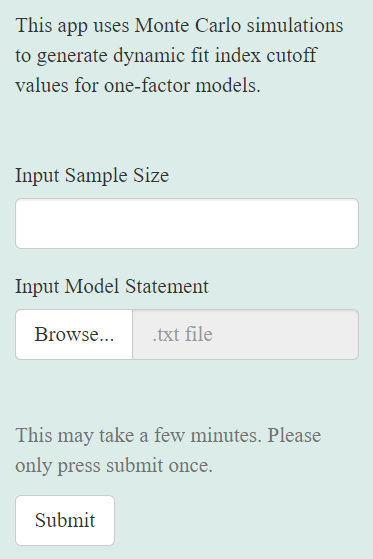
\includegraphics[width=0.4\linewidth]{inputs} 

}

\caption{The required inputs for the one-factor CFA app.}\label{fig:inputs}
\end{figure}

\hypertarget{mplus}{%
\section{Mplus}\label{mplus}}

To get the standardized loadings from Mplus (current as of version 8.7), we add the following argument to the end of the input file: \texttt{OUTPUT:\ STDYX;} . The standardized loadings will be found under the section of the output titled \texttt{STDYX\ STANDARDIZATION} (see Figure \ref{fig:mplus}). The magnitude of the standardized loading for each indicator is under the header titled Estimate. For example, the standardized loading for E1 is .671.

\begin{figure}

{\centering 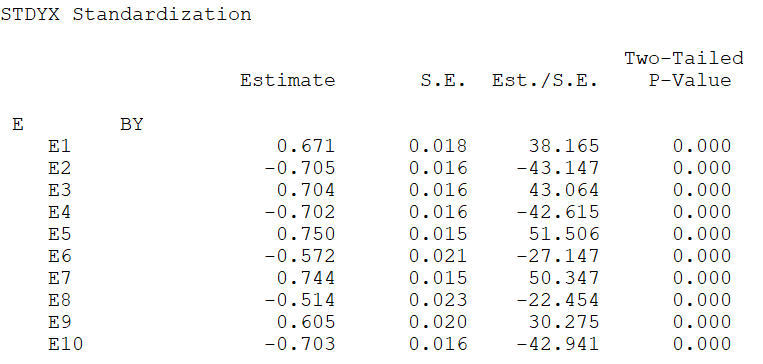
\includegraphics[width=0.7\linewidth]{mplus} 

}

\caption{The standardized loadings from Mplus.}\label{fig:mplus}
\end{figure}

\hypertarget{spss-amos}{%
\section{SPSS Amos}\label{spss-amos}}

To get the standardized loadings from SPSS Amos (current as of version 28), users should select the ``Analysis Properties'' icon, and check the ``Standardized estimates'' box under the ``Output'' tab. After running the model, the standardized loadings can be found in the ``Parameter Formats'' box by deselecting ``Unstandardized estimates'' and selecting ``Standardized estimates''. They will appear on the path diagram and can easily be copied from the syntax. The syntax can be accessed by toggling to the ``Syntax'' tab underneath the path diagram (see Figure \ref{fig:amos}).

\begin{figure}

{\centering 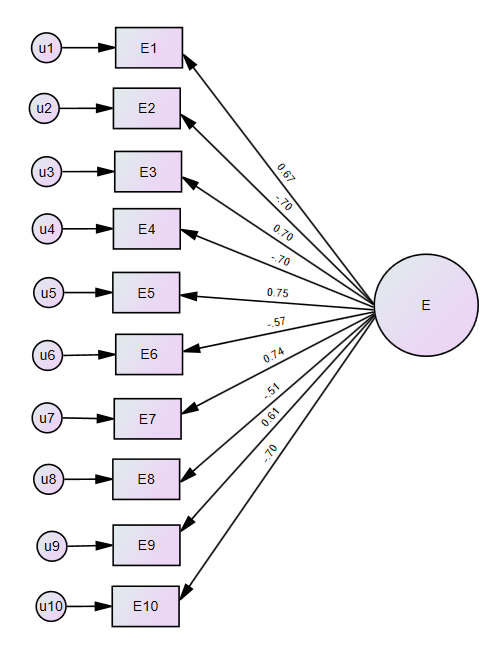
\includegraphics[width=0.5\linewidth]{amos path} 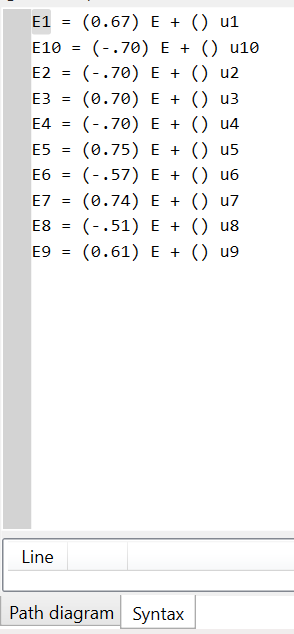
\includegraphics[width=0.3\linewidth]{amos loadings} 

}

\caption{A path diagram with standardized loadings from Amos, and the standardized loadings as seen in the Amos Syntax tab.}\label{fig:amos}
\end{figure}

\hypertarget{model-statement}{%
\section{Model Statement}\label{model-statement}}

We will use the standardized loadings from Mplus and Amos to write out the model statement. Note that the model statement must be saved in a .txt file to be uploaded to the app. The easiest way to create a .txt file on a PC is in Notepad, while the easiest way on a Mac is in TextEdit (make sure to save your TextEdit file as plain text).

The model statement should be written in lavaan style syntax . The regression relationship between the factor and any items will use the syntax =\textasciitilde, while any correlational relationships (e.g., between factors or items) will use the syntax \textasciitilde\textasciitilde. The model statement for this one-factor CFA model will be written as:

\[ Extraversion =~ .671*E1 + -.705*E2 + .704*E3 + -.702*E4 \\ 
+ .750*E5 + -.572*E6 + .744*E7 + -.514*E8 + .605*E9 + -.703*E10 \]

As seen above, the model statement follows the following format: Factor = item loading magnitude * item name. Because the first loading had a magnitude of .671, it is written as .671*E1. The magnitude of the loading will always come before the name of the item. The factors and items can have any name (e.g., orange =\textasciitilde{} .671*apple would work), however the name cannot start with a number (e.g., 123orange would not be permissible). Note that negative loadings still need to have a + sign as a link in the model statement (e.g., .671*E1 + -.705*E2). This model statement would then be saved as a .txt file and uploaded to the app along with the sample size (in this case, the sample size is 1,222). Users would then press submit to begin the simulation.

\hypertarget{levels}{%
\chapter{Why are there different levels and what do they mean?}\label{levels}}

After submitting the model statement and the sample size, the app will compute several Monte Carlo simulations (each with 500 replications) to return the DFI cutoffs. Once the busy bar finishes running, the DFI cutoffs will be found under the ``Results'' tab. For most models, there will be a series of cutoff values beginning with ``Level 1''. One-factor models will typically have three levels of cutoff values . Figure \ref{fig:output-one} displays the three levels of DFI cutoffs for the model used in this tutorial.

\begin{figure}

{\centering 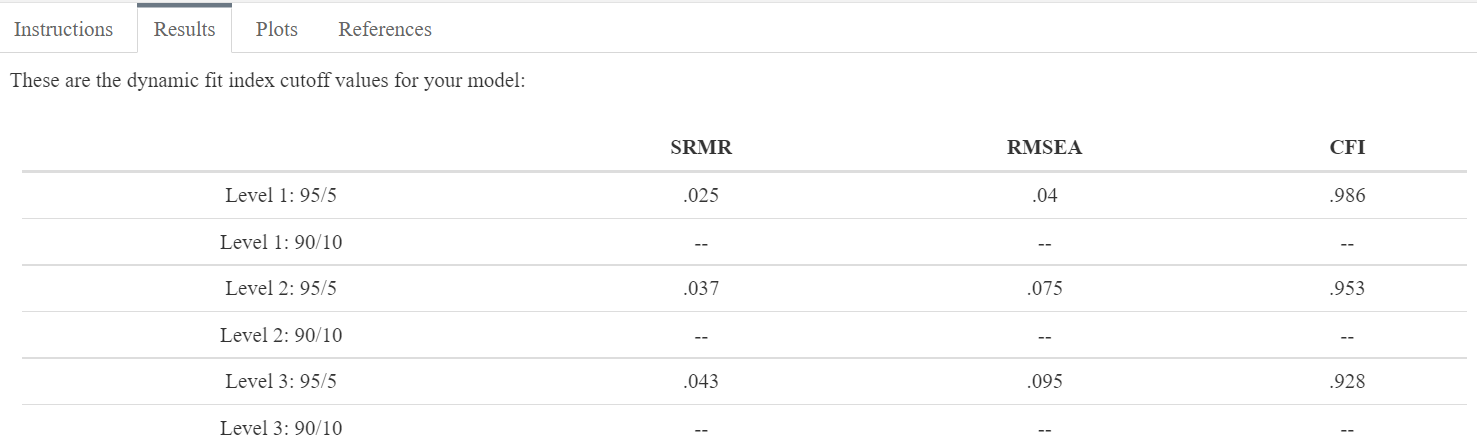
\includegraphics[width=1\linewidth]{one-output} 

}

\caption{The DFI cutoffs for the model used in this tutorial.}\label{fig:output-one}
\end{figure}

The levels correspond to increasing degrees of misspecification in the fit of the model, enabling researchers to reconceptualize misfit as a continuum analogous to an effect size measure. Misspecifications are cumulative such that higher levels are equivalent to more egregious model misspecifications. The Level 1 cutoff can therefore be thought of as the strictest fit criteria because it is consistent with the smallest misspecification from the misfit continuum. Thus, the ideal outcome would be if a user's fitted values for their SRMR, RMSEA, and CFI were all below the Level 1 cutoff, because this would indicate that the observed fitted values were more similar to a model that was correctly specified. In other words, if the user's model fit was below the Level 1 cutoffs, that would mean it fit better than a model that had only a minor misspecification. As the levels increase, the cutoff values will become more lenient because they will correspond to models that are more misspecified.

If the fitted values for a one-factor model were above the Level 1 cutoff but below the Level 2 cutoff, one might conclude that their model was consistent with modest misspecifications and could potentially argue that the misspecifications were not a substantial threat to the validity of their inferences. If the fitted values were above the Level 2 cutoff but below the Level 3 cutoff, the model fit might be categorized as moderately misspecified, while fitted values above the Level 3 cutoff might be described as substantially misspecified. It is also possible to observe fitted values for each of the indices that are classified at differing cutoff levels. In this case, the researcher might report that the fit indices were consistent with different degrees of misspecification, and potentially attempt to diagnose the inconsistencies (e.g., by investigating local areas of strain). As always, it is up to the researcher to present multiple types of evidence in defense of the validity of their assessment (e.g., finding fit consistent with a minor misspecification should not be the entirety of the claim for evidence of validity). See Chapter \ref{algorithm} for more discussion about levels and model misspecification.

\hypertarget{applied-example-1}{%
\section{Applied Example}\label{applied-example-1}}

To determine how well their model fits their data, researchers should compare the fit of their model (derived from their software of choice) to the DFI cutoffs derived from the app or the R package. In this case, the fit index values for the Extraversion empirical model are \({\chi}^2\) = 436.55 (df = 35, p \textless{} .001), SRMR = .048, RMSEA = .097 {[}.089, .105{]}, CFI = .921. Compared to the traditional fixed cutoff values from Hu and Bentler \citeyearpar{hu_cutoff_1999}, the SRMR would be indicative of good fit while the RMSEA and the CFI would be indicative of poor fit.

There are two drawbacks to using the fixed cutoffs. The first is that the fixed cutoffs are derived from a different model subspace (a 3-factor model with 15 items) that does not generalize to our model (a one-factor model with 10 items). The second is that because there is only one set of cutoff values, we cannot infer the degree of misspecification present, forcing us to make a binary decision about a continuum of misspecification. Alternatively, when comparing our fit index values to the DFI cutoffs that are tailored to our empirical model, we see that all three indices are consistent with a Level 3 misspecification (see Figure \ref{fig:output-one}). This is because the SRMR and RMSEA are greater than the Level 3 DFI cutoff, while the CFI is less than the Level 3 DFI cutoff. As such, we can infer that the model is substantially misspecified, rendering it difficult to defend as valid especially without other types of validity evidence. We might follow up by investigating local fit such as consulting the modification indices in our software of choice. In doing so, we see that adding a residual correlation between E8 and E9 would reduce the \({\chi}^2\) by 156.158, or 36\%. The next steps might involve qualitatively investigating the cause of the relationship between these two items, removing one of them if they are deemed redundant, adding a residual correlation between the two of them if it is theoretically justified, or something else.

\hypertarget{ninetyfive}{%
\chapter{What does 95/5 and 90/10 mean, and how should I interpret the plots?}\label{ninetyfive}}

The 95/5 and 9/10 thresholds are derived from Hu and Bentler's approach to minimizing the classification error rates. In Chapter \ref{algorithm}, we mentioned that the DFI algorithm simulates a distribution of fit index values from a correctly specified model and a misspecified model and then selects a cutoff value that distinguishes between the two distributions. In the app, these distributions are visualized under the ``Plots'' tab (see Figure \ref{fig:one-graph} for the Level 3 distributions from the applied example). But how is that value selected, especially when the distributions might overlap leaving researchers unsure as to whether the fit index value that they observed is consistent with one that is derived from a misspecified model or a correctly specified model?

\begin{figure}

{\centering 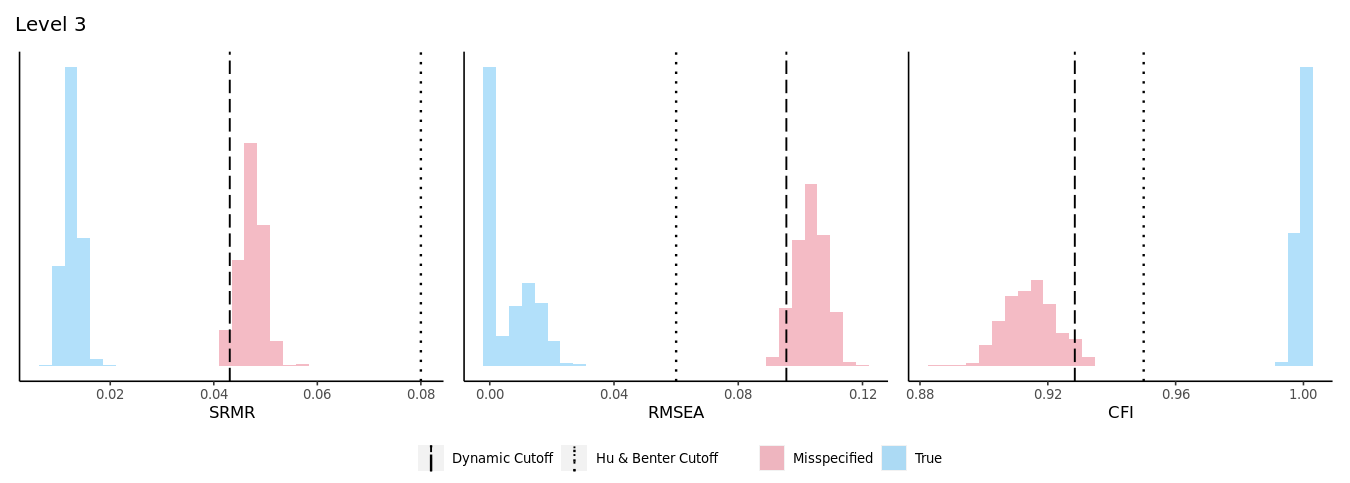
\includegraphics[width=1\linewidth]{one-graph} 

}

\caption{The Level 1 distributions from the DFI algorithm for the Extraversion scale.}\label{fig:one-graph}
\end{figure}

To avoid ambiguity, the DFI algorithm consistently selects the cutoff value from the misspecified distribution. Specifically, the magnitude of the cutoff value corresponds to the 5th percentile of the misspecified distribution for the SRMR and RMSEA and the 95th percentile of the CFI (this is because low values of SRMR and RMSEA are indicative of better fit while high values of CFI are indicative of better fit). These values correspond to the dashed lines in Figure \ref{fig:one-graph} (the Hu and Bentler cutoffs are also presented for comparison as dotted lines). Since the fitted value for the SRMR in the Extraversion example was .048, it is more likely that this value would come from a distribution of misspecified fit indices because the SRMR misspecified distribution (in red) ranges from .041 to .056, while the SRMR correctly specified distribution (in blue) ranges from .008 to .019. As such, the conclusion is that the fitted model is likely misspecified in a way that is consistent with a Level 1 misspecification.

In Figure \ref{fig:one-graph}, the two distributions are distinct and clearly separated. However, sometimes the misspecified and the correctly specified distributions will overlap. Since the distributions can overlap, the rule that the DFI algorithm uses is to select the 5th percentile of the misspecified distribution (for the SRMR and RMSEA) so long as the value that is returned is also greater than the 95th percentile from the correctly specified distribution . This check is put in place to safeguard against mistakenly choosing a cutoff value that could just as easily come from a correctly specified distribution. If the distributions overlap too much, (such that the 5th percentile of the misspecified distribution is less than the 95th percentile of the correctly specified distribution), then the DFI algorithm will attempt to return the 10th percentile of the misspecified distribution so long as the value is greater than the 90th percentile of the correctly specified distribution. Conceptually, this is like changing the alpha from .05 to .10 in standard null hypothesis significance testing. As such, the probability of misclassification is higher with the 90/10 rule than with the 95/5 rule, but the overall likelihood of making an error is still reasonably low \citep{mcneish_dynamic_2022}.

\hypertarget{none}{%
\chapter{What does NONE mean, and what should I do if I see it?}\label{none}}

In Chapter \ref{ninetyfive}, we spoke about how the cutoff values are derived from the 5th percentile of the misspecified distributions of fit indices (for SRMR and RMSEA; the 95th percentile for CFI), and the problems that begin to arise if the misspecified and correctly specified distributions overlap. If the misspecified and correctly specified distributions of fit indices overlap substantially, then we become unsure as to whether an observed fitted value would be more likely to be found in a distribution of fit indices that were derived from a correctly specified model or a misspecified model. An example of this can be seen in Figure \ref{fig:overlap}. When this happens, the DFI algorithm will return the word ``NONE'' for that fit index.

\begin{figure}

{\centering 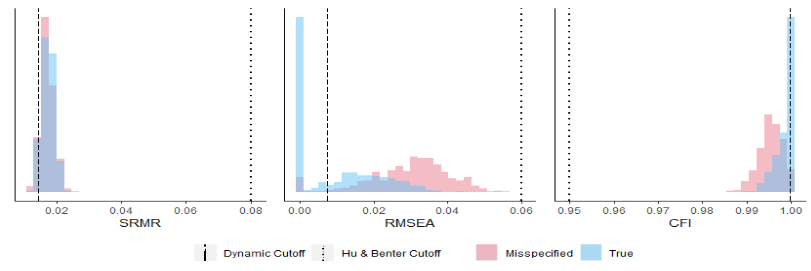
\includegraphics[width=1\linewidth]{overlap} 

}

\caption{An example of overlapping distributions that would result in a NONE outcome.}\label{fig:overlap}
\end{figure}

When the word ``NONE'' is returned, that means that there are no cutoff values for that level of misfit that can reliably distinguish between a correctly specified model and a misspecified model. This can be verified visually in the ``Plots'' tab of the app. This is more likely to happen when sample sizes are small and loadings are low \citep{hancock_reliability_2011, heene_masking_2011, mcneish_thorny_2018}. If there are DFI cutoff values available for other indices or other levels, they can and should still be used. If there are no DFI cutoff values available for any indices or any levels, the solution is not to rely on the traditional fixed cutoff values from Hu and Bentler as they similarly cannot distinguish between a correct and misspecified model. Instead, users can attempt to collect more data to increase their sample size, rely on the \({\chi}^2\) test, or investigate local fit.

\hypertarget{manuscript}{%
\chapter{How do I include DFI cutoffs in a manuscript?}\label{manuscript}}

In our experience, it is easiest to include DFI cutoffs in a manuscript by putting them in a table and then referencing the table in the text of the article. Researchers should report the fit of their model as they normally would, and then reference the likely magnitude of misspecification by comparing each approximate fit index to the table of DFI cutoff values. An example of a write up using the model from this tutorial is presented in the next section. Because tailored cutoffs (specifically, DFI cutoffs) are a relatively new development, it may be worthwhile to mention that they are used to quantify the degree of misfit in the model or include a sentence about the limitations of fixed cutoff values for readers who are not familiar with existing literature.

In this tutorial, the model was substantially misspecified. When this happens, researchers may be interested in modifying the model to attempt to improve the fit (although, note that model modification is only potential resolution and modifications should not be made without strong theoretical justifications). It is not clear to us quite yet how to proceed with DFI cutoffs when using modifying the model (i.e., we are not sure if DFI cutoffs should be updated for the new model or not). This is discussed more in Chapter \ref{limitations}. We are currently working on resolving this conundrum so that we can make clear recommendations for researchers.

\hypertarget{applied-example-standard-reporting}{%
\section{Applied Example: Standard Reporting}\label{applied-example-standard-reporting}}

The test of exact fit was statistically significant (\({\chi}^2\) = 436.55, df = 35, \(p\) \textless{} .001) indicating that the model did not exactly fit the data. The approximate fit indices for the model were SRMR = .048, RMSEA = .097 {[}90\% CI (.089, .105){]}, and CFI = .921. These indices are essentially effect size measure for the magnitude of misfit. To quantify the degree of misfit reflected in these indices is, we compare the fit indices to a series of dynamic fit index (DFI) cutoffs \citep{mcneish_dynamic_2022} calculated by the one-factor DFI Shiny app version 1.1.0 \citep{wolf_dynamic_2020}. A table with the resulting cutoffs derived for this model are shown below. The SRMR and RMSEA from the model were above the Level-3 DFI cutoff and the CFI was below the Level-3 DFI cutoff, indicating that the fit of the model is consistent with a substantial misspecification.

\begin{table}

\caption{\label{tab:tab}The DFI cutoffs used to quantify the degree of misfit in the model.}
\centering
\begin{tabular}[t]{lccc}
\toprule
  & SRMR & RMSEA & CFI\\
\midrule
Level 1 & 0.025 & 0.040 & 0.986\\
Level 2 & 0.037 & 0.075 & 0.953\\
Level 3 & 0.043 & 0.095 & 0.928\\
\bottomrule
\end{tabular}
\end{table}

\hypertarget{nonexist}{%
\chapter{What should I do if DFI cutoffs don't exist for my model type?}\label{nonexist}}

As of this writing, the DFI method supports CFA models with continuous indicators only and the simulation component of the software assumes multivariate normality. It takes some time to work out generalizations for other types of models because a general method for identifying relevant misspecifications must be done model by model. For instance, potential misspecification that are relevant to latent growth models would likely be very different than a confirmatory factor analysis because latent growth models are typically interested in aspects like the function form of growth being correct or whether the correlation between repeated measures is reasonable rather than things like omitted cross-loadings that are relevant to confirmatory factor analysis. Our current work is focused on extending the method to higher-order models, categorical indicators, non-normality, missing data, and measurement invariance; so we expect those or related extensions will be the next to be added to the DFI method.

In the meantime, researchers should rely on the chi-square test and investigate local areas of strain to look for obvious misfit (e.g., viewing the standardized residual covariance matrix). Researchers can also use the Exact Fit application in the Shiny App or the \texttt{exactFit} function in the R package to return the 95th or 99th percentile of the distribution of cutoff values for a correctly specified model (for researchers that used one of the currently available apps, this can also be found in the Level 0 tab). Because this is a distribution of cutoff values for the true model, the values that are returned are the strictest way to evaluate approximate model fit. If the researchers fit index values fall below these values, this indicates that the fit of their model is consistent with a model that is correctly specified. These cutoff values can be computed for any model with continuous outcomes (e.g., models estimated using ML or MLR).

\hypertarget{limitations}{%
\chapter{What are the limitations of DFI cutoffs?}\label{limitations}}

In addition to only being available for a limited number of model types, DFI cutoffs have three other notable limitations. Currently, the cutoff values are derived by simulating data that is multivariate normal, which may not be consistent with the researcher's real data. We are currently working on switching to a bootstrapping approach which would sample the researcher's data and account for any non-normality anywhere in the model, resulting in cutoff values that are more accurate. Implementing this would require researchers to upload their data to the app, but it would mean that the model statement was simpler to write (e.g., it would no longer be necessary to include the magnitude of the standardized loadings in the model statement).

Additionally, the misspecifications for the one-factor model are currently standardized and thus somewhat comparable across models regardless of the number of items, but the misspecifications for the multi-factor models are not. This is because the multi-factor model replicates Hu and Bentler's approach to misspecification which involves adding one cross-loading for each f-1 factor in the model with a magnitude equivalent to the item with the lowest loading in the model. Meanwhile, the one-factor model simply adds residual correlations with magnitudes of .3 proportional to the total number of items in the model. We are also working on introducing a similar standardized approach to model misspecification for multi-factor models.

Lastly, it is not clear to us quite yet if DFI cutoffs should be recomputed every time a model is modified. It is possible that cutoff values could change considerably for multi-factor models if the magnitude of the lowest factor-loading changes substantially (e.g., from .3 to .7). This will likely be resolved by standardizing the approach to misspecification for multi-factor models, which will make it easier to determine if the cutoff values should be recalculated. At this point, we hypothesize that it may not be necessary to recompute DFI cutoffs for small modifications to a model (i.e., adding a residual correlation) but it may be necessary to recompute DFI cutoffs for larger modifications (e.g., switching from a one-factor model to a two-factor model).

  \bibliography{references.bib,packages.bib}

\end{document}
